\documentclass[twoside]{book}

% Packages required by doxygen
\usepackage{calc}
\usepackage{doxygen}
\usepackage{graphicx}
\usepackage[utf8]{inputenc}
\usepackage{makeidx}
\usepackage{multicol}
\usepackage{multirow}
\usepackage{textcomp}
\usepackage[table]{xcolor}

% Font selection
\usepackage[T1]{fontenc}
\usepackage{mathptmx}
\usepackage[scaled=.90]{helvet}
\usepackage{courier}
\usepackage{amssymb}
\usepackage{sectsty}
\renewcommand{\familydefault}{\sfdefault}
\allsectionsfont{%
  \fontseries{bc}\selectfont%
  \color{darkgray}%
}
\renewcommand{\DoxyLabelFont}{%
  \fontseries{bc}\selectfont%
  \color{darkgray}%
}

% Page & text layout
\usepackage{geometry}
\geometry{%
  a4paper,%
  top=2.5cm,%
  bottom=2.5cm,%
  left=2.5cm,%
  right=2.5cm%
}
\tolerance=750
\hfuzz=15pt
\hbadness=750
\setlength{\emergencystretch}{15pt}
\setlength{\parindent}{0cm}
\setlength{\parskip}{0.2cm}
\makeatletter
\renewcommand{\paragraph}{%
  \@startsection{paragraph}{4}{0ex}{-1.0ex}{1.0ex}{%
    \normalfont\normalsize\bfseries\SS@parafont%
  }%
}
\renewcommand{\subparagraph}{%
  \@startsection{subparagraph}{5}{0ex}{-1.0ex}{1.0ex}{%
    \normalfont\normalsize\bfseries\SS@subparafont%
  }%
}
\makeatother

% Headers & footers
\usepackage{fancyhdr}
\pagestyle{fancyplain}
\fancyhead[LE]{\fancyplain{}{\bfseries\thepage}}
\fancyhead[CE]{\fancyplain{}{}}
\fancyhead[RE]{\fancyplain{}{\bfseries\leftmark}}
\fancyhead[LO]{\fancyplain{}{\bfseries\rightmark}}
\fancyhead[CO]{\fancyplain{}{}}
\fancyhead[RO]{\fancyplain{}{\bfseries\thepage}}
\fancyfoot[LE]{\fancyplain{}{}}
\fancyfoot[CE]{\fancyplain{}{}}
\fancyfoot[RE]{\fancyplain{}{\bfseries\scriptsize Generated on Thu Nov 5 2015 23\-:03\-:53 for My Project by Doxygen }}
\fancyfoot[LO]{\fancyplain{}{\bfseries\scriptsize Generated on Thu Nov 5 2015 23\-:03\-:53 for My Project by Doxygen }}
\fancyfoot[CO]{\fancyplain{}{}}
\fancyfoot[RO]{\fancyplain{}{}}
\renewcommand{\footrulewidth}{0.4pt}
\renewcommand{\chaptermark}[1]{%
  \markboth{#1}{}%
}
\renewcommand{\sectionmark}[1]{%
  \markright{\thesection\ #1}%
}

% Indices & bibliography
\usepackage{natbib}
\usepackage[titles]{tocloft}
\setcounter{tocdepth}{3}
\setcounter{secnumdepth}{5}
\makeindex

% Hyperlinks (required, but should be loaded last)
\usepackage{ifpdf}
\ifpdf
  \usepackage[pdftex,pagebackref=true]{hyperref}
\else
  \usepackage[ps2pdf,pagebackref=true]{hyperref}
\fi
\hypersetup{%
  colorlinks=true,%
  linkcolor=blue,%
  citecolor=blue,%
  unicode%
}

% Custom commands
\newcommand{\clearemptydoublepage}{%
  \newpage{\pagestyle{empty}\cleardoublepage}%
}


%===== C O N T E N T S =====

\begin{document}

% Titlepage & ToC
\hypersetup{pageanchor=false}
\pagenumbering{roman}
\begin{titlepage}
\vspace*{7cm}
\begin{center}%
{\Large My Project }\\
\vspace*{1cm}
{\large Generated by Doxygen 1.8.6}\\
\vspace*{0.5cm}
{\small Thu Nov 5 2015 23:03:53}\\
\end{center}
\end{titlepage}
\clearemptydoublepage
\tableofcontents
\clearemptydoublepage
\pagenumbering{arabic}
\hypersetup{pageanchor=true}

%--- Begin generated contents ---
\chapter{Hierarchical Index}
\section{Class Hierarchy}
This inheritance list is sorted roughly, but not completely, alphabetically\-:\begin{DoxyCompactList}
\item \contentsline{section}{Creature}{\pageref{classCreature}}{}
\item \contentsline{section}{Darwin}{\pageref{classDarwin}}{}
\item \contentsline{section}{Instruction}{\pageref{classInstruction}}{}
\item iterator\begin{DoxyCompactList}
\item \contentsline{section}{Darwin\-\_\-\-Iterator}{\pageref{classDarwin__Iterator}}{}
\end{DoxyCompactList}
\item \contentsline{section}{Species}{\pageref{classSpecies}}{}
\end{DoxyCompactList}

\chapter{Class Index}
\section{Class List}
Here are the classes, structs, unions and interfaces with brief descriptions\-:\begin{DoxyCompactList}
\item\contentsline{section}{\hyperlink{classCreature}{Creature} }{\pageref{classCreature}}{}
\item\contentsline{section}{\hyperlink{classDarwin}{Darwin} }{\pageref{classDarwin}}{}
\item\contentsline{section}{\hyperlink{classDarwin__Iterator}{Darwin\-\_\-\-Iterator} }{\pageref{classDarwin__Iterator}}{}
\item\contentsline{section}{\hyperlink{classInstruction}{Instruction} }{\pageref{classInstruction}}{}
\item\contentsline{section}{\hyperlink{classSpecies}{Species} }{\pageref{classSpecies}}{}
\end{DoxyCompactList}

\chapter{Class Documentation}
\hypertarget{classCreature}{\section{Creature Class Reference}
\label{classCreature}\index{Creature@{Creature}}
}


{\ttfamily \#include $<$Creature.\-h$>$}

\subsection*{Public Member Functions}
\begin{DoxyCompactItemize}
\item 
\hyperlink{classCreature_a199600db8c83b460a8fa45487bad6667}{Creature} (const \hyperlink{classSpecies}{Species} \&s=\hyperlink{classSpecies}{Species}(), char d= '?')
\item 
\hypertarget{classCreature_a73ce9f30b95948c44e2224305229c25e}{void {\bfseries print} (int turn=0)}\label{classCreature_a73ce9f30b95948c44e2224305229c25e}

\end{DoxyCompactItemize}
\subsection*{Friends}
\begin{DoxyCompactItemize}
\item 
\hypertarget{classCreature_aae4fdf24dfdd3936f1ba810d44088f64}{class {\bfseries Darwin}}\label{classCreature_aae4fdf24dfdd3936f1ba810d44088f64}

\end{DoxyCompactItemize}


\subsection{Detailed Description}
Interface for Creature.\-c++ 

\subsection{Constructor \& Destructor Documentation}
\hypertarget{classCreature_a199600db8c83b460a8fa45487bad6667}{\index{Creature@{Creature}!Creature@{Creature}}
\index{Creature@{Creature}!Creature@{Creature}}
\subsubsection[{Creature}]{\setlength{\rightskip}{0pt plus 5cm}Creature\-::\-Creature (
\begin{DoxyParamCaption}
\item[{const {\bf Species} \&}]{s = {\ttfamily {\bf Species}()}, }
\item[{char}]{d = {\ttfamily '?'}}
\end{DoxyParamCaption}
)}}\label{classCreature_a199600db8c83b460a8fa45487bad6667}
Constructor. Makes a species and gives it a direction d 

The documentation for this class was generated from the following files\-:\begin{DoxyCompactItemize}
\item 
Creature.\-h\item 
Creature.\-c++\end{DoxyCompactItemize}

\hypertarget{classDarwin}{\section{Darwin Class Reference}
\label{classDarwin}\index{Darwin@{Darwin}}
}


{\ttfamily \#include $<$Darwin.\-h$>$}

\subsection*{Public Member Functions}
\begin{DoxyCompactItemize}
\item 
void \hyperlink{classDarwin_a0d2638a42288b3588dd2edca3f9252e9}{step} (int n=1)
\item 
\hypertarget{classDarwin_a4e33d343a1c2624442c2b7e5ed378053}{\hyperlink{classDarwin__Iterator}{Darwin\-\_\-\-Iterator} {\bfseries begin} ()}\label{classDarwin_a4e33d343a1c2624442c2b7e5ed378053}

\item 
\hypertarget{classDarwin_a4213db821993b8baaa587746335660ea}{\hyperlink{classDarwin__Iterator}{Darwin\-\_\-\-Iterator} {\bfseries end} ()}\label{classDarwin_a4213db821993b8baaa587746335660ea}

\item 
\hypertarget{classDarwin_a5fa1bd92338f783740407ae2bf188f1f}{const \hyperlink{classCreature}{Creature} \& {\bfseries at} (int n)}\label{classDarwin_a5fa1bd92338f783740407ae2bf188f1f}

\item 
\hypertarget{classDarwin_a045d481594ec3a616c266a13cc4b89c2}{{\bfseries Darwin} (int w=1, int h=1)}\label{classDarwin_a045d481594ec3a616c266a13cc4b89c2}

\item 
\hypertarget{classDarwin_aa8ba3b5a820d6bf68888c07be9ff34af}{void {\bfseries add\-Creature} (\hyperlink{classCreature}{Creature} $\ast$, int, int)}\label{classDarwin_aa8ba3b5a820d6bf68888c07be9ff34af}

\item 
void \hyperlink{classDarwin_aa707da4e90db5d6a4e15f8e65f15134f}{print} (ostream \&w, int turn=0)
\end{DoxyCompactItemize}
\subsection*{Friends}
\begin{DoxyCompactItemize}
\item 
\hypertarget{classDarwin_a45a59c9aa68fc4c29a090ee25b3745b9}{class {\bfseries Darwin\-\_\-\-Iterator}}\label{classDarwin_a45a59c9aa68fc4c29a090ee25b3745b9}

\end{DoxyCompactItemize}


\subsection{Detailed Description}
Interface for Darwin.\-c++ 

\subsection{Member Function Documentation}
\hypertarget{classDarwin_aa707da4e90db5d6a4e15f8e65f15134f}{\index{Darwin@{Darwin}!print@{print}}
\index{print@{print}!Darwin@{Darwin}}
\subsubsection[{print}]{\setlength{\rightskip}{0pt plus 5cm}void Darwin\-::print (
\begin{DoxyParamCaption}
\item[{ostream \&}]{w, }
\item[{int}]{turn = {\ttfamily 0}}
\end{DoxyParamCaption}
)}}\label{classDarwin_aa707da4e90db5d6a4e15f8e65f15134f}
Prints the grid with numbers and letters as indicies \hypertarget{classDarwin_a0d2638a42288b3588dd2edca3f9252e9}{\index{Darwin@{Darwin}!step@{step}}
\index{step@{step}!Darwin@{Darwin}}
\subsubsection[{step}]{\setlength{\rightskip}{0pt plus 5cm}void Darwin\-::step (
\begin{DoxyParamCaption}
\item[{int}]{n = {\ttfamily 1}}
\end{DoxyParamCaption}
)}}\label{classDarwin_a0d2638a42288b3588dd2edca3f9252e9}
Does the actions of the creature and makes sure they don't act twice 

The documentation for this class was generated from the following files\-:\begin{DoxyCompactItemize}
\item 
Darwin.\-h\item 
Darwin.\-c++\end{DoxyCompactItemize}

\hypertarget{classDarwin__Iterator}{\section{Darwin\-\_\-\-Iterator Class Reference}
\label{classDarwin__Iterator}\index{Darwin\-\_\-\-Iterator@{Darwin\-\_\-\-Iterator}}
}
Inheritance diagram for Darwin\-\_\-\-Iterator\-:\begin{figure}[H]
\begin{center}
\leavevmode
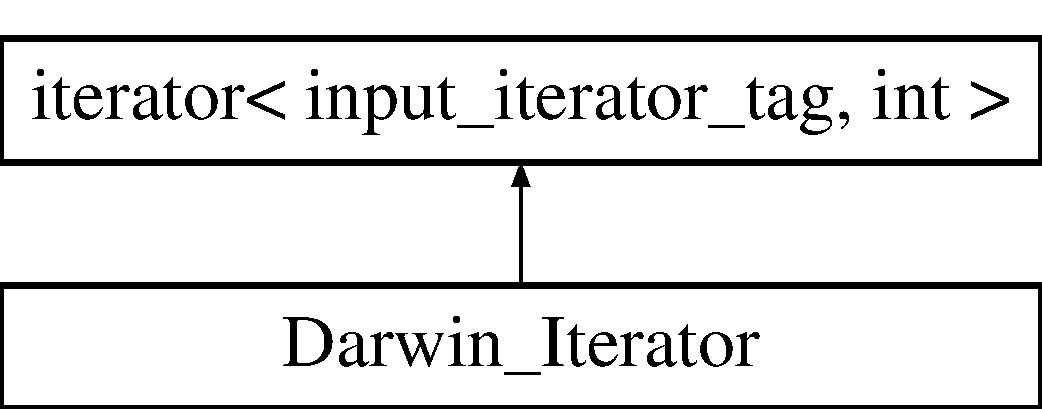
\includegraphics[height=2.000000cm]{classDarwin__Iterator}
\end{center}
\end{figure}
\subsection*{Public Member Functions}
\begin{DoxyCompactItemize}
\item 
\hypertarget{classDarwin__Iterator_a213a26bffa63a58803d96a13350acf28}{{\bfseries Darwin\-\_\-\-Iterator} (int v, \hyperlink{classDarwin}{Darwin} $\ast$dar)}\label{classDarwin__Iterator_a213a26bffa63a58803d96a13350acf28}

\item 
\hypertarget{classDarwin__Iterator_a6f7e8d9dd3d46d5e24e714cf63905a2c}{bool {\bfseries operator==} (const \hyperlink{classDarwin__Iterator}{Darwin\-\_\-\-Iterator} \&rhs) const }\label{classDarwin__Iterator_a6f7e8d9dd3d46d5e24e714cf63905a2c}

\item 
\hypertarget{classDarwin__Iterator_a1d4d68e28d1eee5c8361d8a38e9192f2}{bool {\bfseries operator!=} (const \hyperlink{classDarwin__Iterator}{Darwin\-\_\-\-Iterator} \&rhs) const }\label{classDarwin__Iterator_a1d4d68e28d1eee5c8361d8a38e9192f2}

\item 
\hypertarget{classDarwin__Iterator_aa36cdd2af8ed99f148feaf0fb36afee3}{const \hyperlink{classCreature}{Creature} \& {\bfseries operator$\ast$} () const }\label{classDarwin__Iterator_aa36cdd2af8ed99f148feaf0fb36afee3}

\item 
\hypertarget{classDarwin__Iterator_a19c7a708eb76cae5b6ad345a80702380}{\hyperlink{classDarwin__Iterator}{Darwin\-\_\-\-Iterator} \& {\bfseries operator++} ()}\label{classDarwin__Iterator_a19c7a708eb76cae5b6ad345a80702380}

\item 
\hypertarget{classDarwin__Iterator_a4dbff05c6e280513fc8a09093409afa5}{\hyperlink{classDarwin__Iterator}{Darwin\-\_\-\-Iterator} {\bfseries operator++} (int)}\label{classDarwin__Iterator_a4dbff05c6e280513fc8a09093409afa5}

\end{DoxyCompactItemize}


The documentation for this class was generated from the following file\-:\begin{DoxyCompactItemize}
\item 
Darwin.\-h\end{DoxyCompactItemize}

\hypertarget{classInstruction}{\section{Instruction Class Reference}
\label{classInstruction}\index{Instruction@{Instruction}}
}


{\ttfamily \#include $<$Instruction.\-h$>$}

\subsection*{Public Member Functions}
\begin{DoxyCompactItemize}
\item 
\hypertarget{classInstruction_af0047418ce174426a4f3bdf48304db8e}{virtual pair$<$ int, char $>$ {\bfseries act} (char, char, char, char, int, char)=0}\label{classInstruction_af0047418ce174426a4f3bdf48304db8e}

\end{DoxyCompactItemize}


\subsection{Detailed Description}
Interface for the individual instructions 

The documentation for this class was generated from the following file\-:\begin{DoxyCompactItemize}
\item 
Instruction.\-h\end{DoxyCompactItemize}

\hypertarget{classSpecies}{\section{Species Class Reference}
\label{classSpecies}\index{Species@{Species}}
}


{\ttfamily \#include $<$Species.\-h$>$}

\subsection*{Public Member Functions}
\begin{DoxyCompactItemize}
\item 
\hypertarget{classSpecies_a85b7ef8c3c760f3a8f5888f451bf6274}{{\bfseries Species} (string n=\char`\"{}null\char`\"{})}\label{classSpecies_a85b7ef8c3c760f3a8f5888f451bf6274}

\item 
void \hyperlink{classSpecies_a3b2ef0ea9008e6ccae5599db76c8b5e3}{add\-Instruction} (\hyperlink{classInstruction}{Instruction} $\ast$)
\end{DoxyCompactItemize}
\subsection*{Friends}
\begin{DoxyCompactItemize}
\item 
\hypertarget{classSpecies_a61c90c9560acd7d537ef938505c429c0}{class {\bfseries Creature}}\label{classSpecies_a61c90c9560acd7d537ef938505c429c0}

\item 
\hypertarget{classSpecies_aae4fdf24dfdd3936f1ba810d44088f64}{class {\bfseries Darwin}}\label{classSpecies_aae4fdf24dfdd3936f1ba810d44088f64}

\end{DoxyCompactItemize}


\subsection{Detailed Description}
Interface for Species.\-c++ 

\subsection{Member Function Documentation}
\hypertarget{classSpecies_a3b2ef0ea9008e6ccae5599db76c8b5e3}{\index{Species@{Species}!add\-Instruction@{add\-Instruction}}
\index{add\-Instruction@{add\-Instruction}!Species@{Species}}
\subsubsection[{add\-Instruction}]{\setlength{\rightskip}{0pt plus 5cm}void Species\-::add\-Instruction (
\begin{DoxyParamCaption}
\item[{{\bf Instruction} $\ast$}]{inst}
\end{DoxyParamCaption}
)}}\label{classSpecies_a3b2ef0ea9008e6ccae5599db76c8b5e3}
Adds an instruction to the vector of instructions 

The documentation for this class was generated from the following files\-:\begin{DoxyCompactItemize}
\item 
Species.\-h\item 
Species.\-c++\end{DoxyCompactItemize}

%--- End generated contents ---

% Index
\newpage
\phantomsection
\addcontentsline{toc}{chapter}{Index}
\printindex

\end{document}
